%%%%%%%%%%%%%%%%%%%%%%%%%%%%%%%%%%%%%%%%%%%%%%%%%%%%%%%%%%%%%%%%%%%%%%%%%%%%%
%
%  System        : 
%  Module        : 
%  Object Name   : $RCSfile$
%  Revision      : $Revision$
%  Date          : $Date$
%  Author        : $Author$
%  Created By    : Robert Heller
%  Created       : Thu Nov 8 16:32:25 2018
%  Last Modified : <181110.1313>
%
%  Description 
%
%  Notes
%
%  History
% 
%%%%%%%%%%%%%%%%%%%%%%%%%%%%%%%%%%%%%%%%%%%%%%%%%%%%%%%%%%%%%%%%%%%%%%%%%%%%%
%
%    Copyright (C) 2018  Robert Heller D/B/A Deepwoods Software
%			51 Locke Hill Road
%			Wendell, MA 01379-9728
%
%    This program is free software; you can redistribute it and/or modify
%    it under the terms of the GNU General Public License as published by
%    the Free Software Foundation; either version 2 of the License, or
%    (at your option) any later version.
%
%    This program is distributed in the hope that it will be useful,
%    but WITHOUT ANY WARRANTY; without even the implied warranty of
%    MERCHANTABILITY or FITNESS FOR A PARTICULAR PURPOSE.  See the
%    GNU General Public License for more details.
%
%    You should have received a copy of the GNU General Public License
%    along with this program; if not, write to the Free Software
%    Foundation, Inc., 675 Mass Ave, Cambridge, MA 02139, USA.
%
% 
%
%%%%%%%%%%%%%%%%%%%%%%%%%%%%%%%%%%%%%%%%%%%%%%%%%%%%%%%%%%%%%%%%%%%%%%%%%%%%%

\section{Hello World}

Typically, the first program a programmer writes is one that prints a simple 
message.  The first program in the \textit{C Programming Language} by  Brian 
W. Kernighan and Dennis M. Ritchie is a program that prints ``Hello World'' on 
the computer console.  This first piece actually does this, in 12 different 
languages.  Touch a foil covered country on the map of the world and see 
``Hello World'' displayed on the small screen located in the middle of the 
North Atlantic Ocean in the language of the country you touched.

\subsection*{Processing Element}

This piece uses an Adafruit Feather M0 Express.

\subsection*{Components of Note}

\begin{itemize}
\item Adafruit MPR121 Breakout, a twelve channel I2C touch sensor.
\item Nokia 5110/3310 Monochrome LCD, a small Monochrome LCD, available from 
Adafruit.
\end{itemize}

\subsection*{Documentation}

Schematic and circuit layout information is available on line at 
\url{https://github.com/RobertPHeller/InteractiveArt/tree/master/HelloWorld}.\marginpar{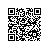
\includegraphics{HelloWorld/HelloWorldonGitHub.png}}

\subsection*{Additional Reading}

\begin{itemize}
\item \textit{Adafruit MPR121 12-Key Capacitive Touch Sensor Breakout
Tutorial} at
\url{https://learn.adafruit.com/adafruit-mpr121-12-key-capacitive-touch-sensor-breakout-tutorial}
\marginpar{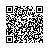
\includegraphics{HelloWorld/mpr121-12-key-capacitive-touch-sensorQR.png}}
\item \textit{Nokia 5110/3310 Monochrome LCD} at
\url{https://learn.adafruit.com/nokia-5110-3310-monochrome-lcd} 
\marginpar{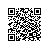
\includegraphics{HelloWorld/nokia-5110-3310-monochrome-lcdQR.png}}
\end{itemize}
